\section{Introducción}
El cáncer de piel es una enfermedad de carácter más o menos grave, según el tipo de tumor al que dé lugar. \\
El melanoma es un tipo de cáncer de piel que se origina cuando los melanocitos (las células responsables de la pigmentación normal de la piel) comienzan a crecer fuera de control. El melanoma es mucho menos frecuente que otros tipos de cánceres de piel, aunque es el más peligroso y agresivo porque evoluciona muy rápidamente, es de fácil diseminación por el organismo y muchas veces mortal si no es detectado en una fase temprana. 
\bigskip

%\begin{wrapfigure}{l}{0.80\textwidth}
%\centering
%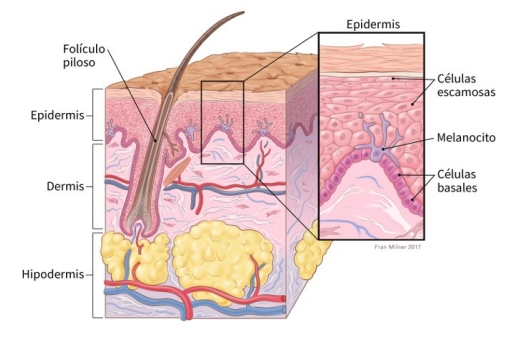
\includegraphics[width=\linewidth]{figures/skin.png}
%\caption{Esquema de las tres capas de la piel}
%\end{wrapfigure}
\begin{tabular}{|cl|cl|}
IMAGEN DE CAPAS DE PIEL 
\end{tabular}

\pagestyle{fancy}
\fancyhf{}
\fancyhead[L]{1. INTRODUCCIÓN}
\newpage
Muchos tipos de tumores benignos (no cancerosos) se pueden originar de los diferentes tipos de células de la piel. Un lunar es un tumor benigno de la piel que también se origina a partir de los melanocitos. No obstante, casi todos los lunares son inofensivos, aunque algunos tipos pueden aumentar su riesgo de melanoma. \\
Un tipo de lunar que a veces se parece al melanoma se llama “nevo Spitz”. Este lunar es más común en niños y adolescentes, aunque a veces se presenta en adultos. Por lo general, estos tumores son benignos y no se propagan. Sin embargo, en ocasiones los médicos tienen problemas para distinguir entre un “nevo Spitz” y un melanoma, aun cuando los observan con un microscopio.

En general, las variedades de melanoma se caracterizan por su Asimetría, Borde irregular, Color heterogéneo, Diámetro grande ($<$ 6mm) y Evolución rápida, también conocido como la regla del ABCDE.
Se reconocen actualmente como factores de riesgo de melanoma: 
\bigskip

\begin{tabular}{|cl|cl|}
TABLA DE CAUSAS
\end{tabular}

\bigskip
Según la etapa del cáncer y otros factores, las opciones de tratamiento podrían incluir: cirugía, inmunoterapia, medicamentos de terapia, quimioterapia, radioterapia para el cáncer de piel tipo melanoma, entre otros.
